\cotefile{66}
\scanpage{2}
\noindent\begin{minipage}[t]{.10\linewidth}
\figure{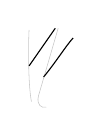
\begin{tikzpicture}[x=.28cm,y=.28cm]
\draw[gray!45,very thin] (.14,3.5) .. controls (.09,2.5) and (.12,.85) .. (.25,.25);
\draw (.14,1.87) -- (1.33,3.58);
\draw[gray!45,very thin] (1.46,3.58) -- (.57,.52) .. controls (.46,.1) and (.71,-.06) .. (.92,0);
\draw (.80,1.37) .. controls (1.34,2.02) and (1.81,2.78) .. (2.14,3.14);
\end{tikzpicture}}
\end{minipage}\hspace{.02\linewidth}%
\begin{minipage}[t]{.86\linewidth}
\tikz[baseline=(yr.base)]{\node[inner sep=2pt] (yr) {1964}; \draw (yr.north west) -- (yr.south west) -- (yr.south east) -- (yr.north east);}
\hfill Numéros cerclés sont sans doute difficiles.

\uline{Travaux de thèses}

\deleted{[\unsure{Collection} \unsure{1964}]}
\end{minipage}%
\begingroup\setlength{\marginparwidth}{2.9cm}\margin{(N.B. Les sujets 1 à 10 et 20, 21, \inserted{26, 27, 28} sont de nature essentiellement cohomologique \unsure{$\zeta$|$\xi$|§|$g$}. 10, 19, 23, 24, 25 \unsure{relèvent|relévent} de la théorie des intersections ; 11, 12, 13 se \unsure{rattachent} à la th. de Néron. 14, 15, 22 th. du topos...; 17, 18 yoga de \unsure{représentabilité}, \unsure{de|des} foncteurs)}\endgroup

1) Topologie et cohomologies $\mathrm{fppf}$ : formalisme \unsure{général|general}
\inserted{\textcircled{\scriptsize $*$} [Rela\uline{tion avec \unsure{coh-mologie|coho-mologie|cohomologie} cristall}ine]}

\reversemarginpar
\textcircled{2}\margin{[subordonné à 1), 11)]} \rule[.45ex]{3.9em}{.45pt} : dualité (\uline{locale}, globale).

\textcircled{3}\margin{[subordonné à 2), donc à 1) et 11)]} Partie $p$-primaire dans formule de Ogg-\unsure{Chafarévitch|Chafovévitch}

\normalmarginpar
\textcircled{4} Formule de RR en cohomologie étale, coeff. discrets.
\unsure{Relation|Relations} avec \unsure{représentation|représentations} d'Artin supérieures.
\inserted{[Formule du $\unsure{\chi|x}$ pour revêtement étale d'un schéma propre...]\unsure{.}}

5) Formule du $\chi$ pour V.A. avec anneau d'opérateurs (variante de Ogg-\unsure{chafarévitch}).

6) Formules de Lefschetz explicites (coeff. discrets étales, ou ``continus'' cohérents). Représentations d'Artin du point de vue cohérent....

\textcircled{7} Cohomologie des schémas de type fini sur $\mathbb{Z}$ ; théorèmes de dualité globale \unsure{satisfaisant|satisfaisants} (améliorant Artin).

\textcircled{8} \unsure{Formalisme|Formalismes} de dualité, du point de vue \inserted{complexes d'}opérateurs différentiels. Coefficients à connexion\unsure{..} intégrable .... \inserted{Lien avec ``cristaux''.}

\textcircled{9} Dualité analytique....

\tikz[baseline=(num.base)]{\node[draw,circle,inner sep=.7pt] (num) {\shortstack{10\\[-.5ex]\scriptsize$\unsure{\times|*}$}};}
Riemann-Roch et \unsure{pbs} connexes (faisceaux pseudo-cohérents de Modules), \inserted{\unsure{analytique|analytiques} ou algébrique.} \inserted{(\unsure{Cf|cf} SGA 6)}

\textcircled{\small 11} Structures et groupes de la catégorie des schémas morcelés. Foncteur de Néron relatif à un anneau de val. discrète.
% archive sheet number: 1

\scanpage{3}
\reversemarginpar
12)\margin{\unsure{commencé} par Raynaud}% slanted
\hspace{.4em}Mise au point, et extensions diverses, de la théorie des modèles de Néron. \hfill
\begin{minipage}[c]{1.8em}\figure{\tikz[baseline=-.35ex,x=1ex,y=1ex]{\draw (.1,2) -- (0,-.5); \draw (.36,1.85) -- (.24,-.45);}}\end{minipage}

\textcircled{\small 13}\margin{S'impose moins depuis les résultats d'approximation d'Artin}% slanted
\hspace{.4em}\unsure{Théorémes|Théorèmes} \unsure{assymptotiques|asymptotiques} pour les \unsure{foncteurs} de Greenberg, relatifs à un anneau local \unsure{noeth} complet ou hensélien.

14) Structures des Topos (questions d'existence de foncteurs fibres....). Structure des champs champs représentables.... \hfill
\begin{minipage}[c]{1.8em}\figure{\tikz[baseline=-.4ex,x=1ex,y=1ex]{\draw[double,double distance=.3pt] (.7,2) -- (1,2.1) -- (.46,-1) -- (.13,-.65);}}\end{minipage}

\textcircled{\small 15}\margin{fait partiellement par \unsure{Mazur}-Artin. Réflexions de Quillen \unsure{en} train}% slanted
\hspace{.4em}\unsure{Théorie|Théories} du \deleted{\unsure{g}}type d'homotopie des Topos, incluant une définition des $\pi_{\unsure{i|\bullet|\cdot}}$ à \deleted{\unsure{coefficients}} \unsure{noveaux|noyaux|nouveaux} infinitésimaux. \inserted{\unsure{Th's|Thés} d'\unsure{Hurwisz|Hurwicz}. Suites exactes d'homotopie. \unsure{Ths|Thés} de comparaison, \deleted{de \unsure{spécialisation}.}}

\textcircled{\small 16}\margin{contre-exemple de Artin, \unsure{situation} peu engageante}% slanted
\hspace{.4em}\deleted{Théorie de spécialisation du} \inserted{``vrai''} \deleted{groupe fondamental, pour une famille de courbes.} \hfill
\begin{minipage}[c]{1.8em}\figure{\tikz[baseline=-.4ex,x=1ex,y=1ex]{\draw (.75,1.65) -- (1,1.65) -- (.67,-.8) -- (.48,-.65);}}\end{minipage}

17)\margin{\unsure{résolu} par Raynaud \(\bigl[\)}% slanted
\hspace{.4em}\deleted{Séparation de foncteurs : classes de correspondance.... Cas de représentabilité et de non représentabilité de \mbox{$\underline{\mathrm{Pic}}_{X/S}$}, \mbox{$X$} de dim} \deleted{\unsure{de|rel}} \deleted{relative \mbox{$1$} sur \mbox{$S$}.}

\textcircled{\small 18} Question du \unsure{passage} au quotient dans cas artinien et de l'effectivité de données de descente plates. \deleted{\unsure{Construction|Constructions} \unsure{générale|générales} de corps de \unsure{modules|variables}.} \hfill
\begin{minipage}[c]{1.8em}\figure{\tikz[baseline=-.4ex,x=1ex,y=1ex]{\draw[double,double distance=.25pt] (.9,1.8) .. controls (1,1.4) and (.7,0) .. (.31,-.8) -- (.08,-.5);}}\end{minipage}

\tikz[baseline=(num.base)]{\node[draw,circle,inner sep=.7pt] (num) {\shortstack{19\\[-.5ex]\scriptsize$\unsure{\times|*}$}};}
Théorie d'\unsure{amplitude|amplitudes} pour cycles de dim. quelconque.
% archive sheet number: 2
\normalmarginpar

\scanpage{4}
\reversemarginpar
\textcircled{\small 20} Vanishing theorem. Cas des espaces homogènes.

\textcircled{\small 21} $H^{*}(X,F)\to H^{\unsure{*|x}}(X_{0},F_{0})$ ($X_{0}$ fermé dans $X$\inserted{\unsure{coh.|ch.} étale}), quand est-ce un isom ? Suffit-il que ce soit vrai en dim $0$ ? Cas $X=\operatorname{Spec} A$, $X_{0}=\unsure{\operatorname{Spe}|\operatorname{Spec}|\operatorname{Sp}} A/\unsure{I|J}$, $A$ $I$-adique séparé complet. Cas de la localisation étale le long de $X_{0}\subset X$, $X$ affine.

22)\margin{travail \unsure{Saavedra} en train}% slanted
\hspace{.4em}Structure des catégorielles abéliennes avec produit tensoriel $\pm$ rigide, en termes de \unsure{représentation|représentations} linéaires des groupes proalgébriques, et de \unsure{représentation|représentations} de gerbes.... \inserted{(préliminaire algébrique à \unsure{le|la} théorie des motifs).}

\figure{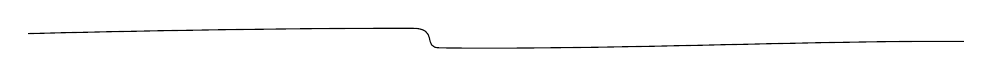
\begin{tikzpicture}[x=.98\linewidth,y=1ex]\draw (0,0) .. controls (.18,.35) and (.32,.45) .. (.41,.45) .. controls (.44,.45) and (.42,-1.2) .. (.44,-1.2) .. controls (.63,-1.35) and (.83,-.6) .. (1,-.65);\end{tikzpicture}}
\par\noindent\uline{Pour \unsure{memoire|mémoire}}

\diagram{\resizebox{\linewidth}{!}{\begin{tikzcd}[ampersand replacement=\&,column sep=2.2em,row sep=0pt,cells={nodes={inner sep=0pt}}]
{\left.\begin{array}{@{}l@{}}
\otimes\ \text{\unsure{Résolution|Résoluton} des singularités.}\\[.8ex]
\otimes\ \text{Pureté cohomologique.}\\[.8ex]
\text{Changement de base régu}\overset{\text{\scriptsize\unsure{?}}}{\text{li}}\text{er}\\[-.3ex]
\qquad\text{\inserted{en cohomologie.}}
\end{array}\right\}}
\arrow[r,Rightarrow,yshift=1.1em]
\arrow[r,Rightarrow,yshift=-1.2em]
\& {\begin{array}{@{}l@{}}
\text{dualité locale}=\text{bidualité,}\\[-.3ex]
\qquad\text{pour la top étale}\\[.8ex]
\text{\unsure{th|ths} de finitude pour morphisme}\\[-.3ex]
\qquad\text{\inserted{de type fini}}\\[-.3ex]
\text{etc etc}
\end{array}}
\end{tikzcd}}}

Dimension cohomologique des \unsure{morphismes} affines.

$\otimes$ \unsure{Théorème|Théorèmes} de finitude genre Grauert.

$\otimes$ Théories \deleted{\unsure{rig|rigide}} type rigide-analytiques.

Questions dans SGA \unsure{1961|1962}

\figure{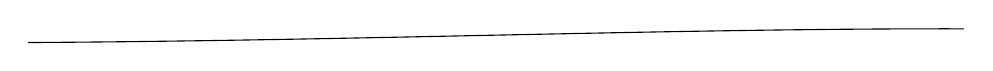
\begin{tikzpicture}[x=.98\linewidth,y=1ex]\draw (0,0) .. controls (.35,.15) and (.7,1.2) .. (1,1.15);\end{tikzpicture}}

\shortstack{23)\\[-.5ex]\scriptsize$\unsure{\times|*}$} Théorie de Chow pour Schémas \deleted{\unsure{qq|qcq} réguliers} ayant un faisceau inversible ample (équivalence rationnelle \unsure{des|de}\unsure{,} cycles). L'image inverse par $f:\unsure{X'|X}\to Y$ doit être définie, sous seule condition que $Y$ soit régulier.

\tikz[baseline=(num.base)]{\node[draw,circle,inner sep=.7pt] (num) {\shortstack{24\\[-.5ex]\scriptsize$\times$}};}
\margin{Réponse négative Griffiths pour question 1\textsuperscript{o}}% slanted
\hspace{.4em}Sur une variété projective lisse connexe de dim $3$ sur $k$ corps \unsure{algébriqmt|algébriquemt|algébriquement} \unsure{clos|clés}, un $1$-cycle num. équiv. à $0$ est-il $\unsure{\tau|t}$-équivalent à zéro ? \inserted{En dim $4$, cycle de dim $2$ équiv. num $=$ équiv. hom ??\unsure{,|'}}
% archive sheet number: 3
\normalmarginpar

\scanpage{5}
\par\noindent\begin{minipage}[t]{.1\linewidth}
\figure{\begin{tikzpicture}[x=.34cm,y=.34cm]
\draw[gray!65,line width=.65pt] (0,0) -- (.4,.5) (.65,.85) -- (1.5,2.08) (1.74,2.4) -- (2.58,3.52);
\draw[gray!65,line width=.65pt] (1.65,-.62) -- (1.9,-.27) (2.17,.09) -- (2.82,.91) (3.62,2.02) -- (3.94,2.43);
\draw[gray!35] (2.99,-.46) .. controls (3.86,-1.34) and (4.05,-.25) .. (4.39,1.11);
\end{tikzpicture}}
\end{minipage}\hspace{.012\linewidth}%
\reversemarginpar
\noindent\tikz[baseline=(num.base)]{\node[draw,circle,inner sep=.6pt] (num) {\shortstack{25\\[-.5ex]\scriptsize$\unsure{\times|*}$}};}\quad Le produit de deux cycles alg. \unsure{èquiv|équiv} à $0$ est-il rat. équiv. à $0$ ? (``pb du carré''). Un $0$-cycle \margin{faux, cf Mumford...\enspace\tikz[baseline=-.4ex,x=.12cm,y=.12cm]{\draw[gray] (.5,2.1) .. controls (-.1,.4) and (0,-.3) .. (.65,-.7) (.62,-.9) -- (.65,-2.3);}}% slanted
qui est alb. èquiv. à $0$ est-il rationnellement \unsure{èquivalent|équivalent} à $0$ ? Question de l'\unsure{équivalence|èquivalence} rationnelle des $0$-cycles sur une surface.
\normalmarginpar

\noindent 26\quad Théorie de Rosenlicht \unsure{relative|reletive} (sur base quelconque)

\noindent 27\quad \unsure{Adèles|Adéles} des schémas de dim\unsure{,|.} quelconque. Jacobiennes locales,

\noindent\tikz[baseline=(num.base)]{\node[draw,circle,inner sep=1pt] (num) {28};}\quad Construction d'une théorie abstraite des motifs sur \unsure{prèschémas|préschémas} de type fini sur $\mathbb{Z}$ (construction catégorique générale),

% archive sheet number: 4

